\section{Design and Implementation}
Throughout this project, rapid prototyping technologies have been used extensively in the design and implementation stage. With very few exceptions, all of the mechanical components that were manufactured were done so by a 3D printer using \gls{PLA} - and even some machine components were first prototyped and tested using printed models.
\newline
A stellar advantage of 3D printing technology is that each of the unique mechanical components used on Tiberius III could be designed and manufactured by ourselves, which was much more convenient than outsourcing the work to other departments. Once a component passed the design stage, it could be quickly manufactured, fitted and tested, and any changes that were required could easily be amended. This was especially useful during the design of the steering and suspension as this was not only a complex mechanical unit, but also needed to be strong enough to support the stresses that the robot would undertake as it explored its environment. Some of the load-bearing parts would have to be manufactured from stronger materials, which would take more time - but 3D printed prototypes could be made first for testing, thus eliminating the risk of a faulty design being sent for manufacture.
\subsection{Wheel and Suspension}
\begin{figure}[!htb]
\begin{center}
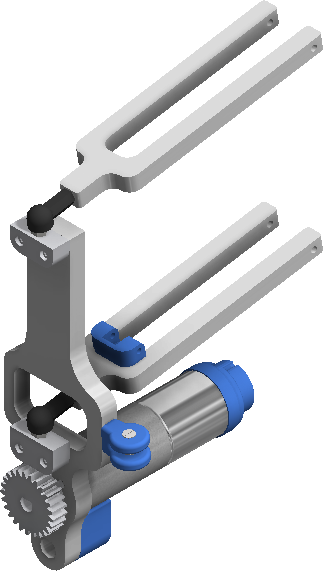
\includegraphics[height=8.5cm]{mech_knuckle.png}
\end{center}
\caption{The steering knuckle, wishbones and motor. 3D printed components in blue.}
\label{fig:mech_knuckle}
\end{figure}
As discussed in Section \ref{sec:Mech_BGT_Steer}, it was decided that Tiberius III would utilise a double-wishbone suspension system. Two wishbones hinged on the robot's chassis would be connected to a steering knuckle with universal ball joints. This steering knuckle - a large piece holding both the wheel and motor - would be able to rotate as Tiberius steers. A colour render of the steering knuckle, with the wishbones and motor fitted, is shown in Figure \ref{fig:mech_knuckle}.
\newline
The steering knuckle holds the new DC motor, which uses two large gears to transfer power to the wheels. This design was chosen as it allows the knuckle to hold the wheel axle on its own, thus none of Tiberius' weight will be resting on the motor shaft. Raising the motor above the wheel also improves the ground clearance, a problem that was discussed in Section \ref{sec:Mech_IP_Tib2}. This has lead to a unique double wishbone design in which both wishbones are located above the wheel axle, instead of one above and one below.
\newline
The shock absorbers used in the suspension were an interesting project in themselves. Purchasing complete suspension units was out of the question, as these could cost hundreds of pounds apiece. The only sensible option was to 3D print these too.
\newline
The suspension unit  is a simple piston-like design, with a linear bearing encased inside two halves of a 3D printed cylinder. The piston shaft - a steel bar with a collar on one end, enclosed inside the piston - can slide in and out. A second collar outside the cylinder holds a plastic plate in place. A large spring is then lodged between the cylinder and this plate. A big advantage of these movable plates is that the compressive force of the shock absorber can be fine-tuned. A colour render of the shock absorber is shown in Figure \ref{fig:mech_piston}.
\begin{figure}[!htb]
\begin{center}
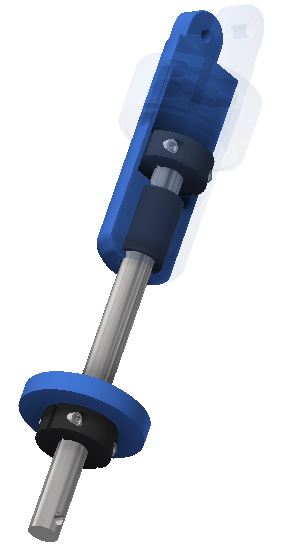
\includegraphics[height=8cm]{mech_piston.png}
\end{center}
\caption{The piston assembly, shown with spring removed.}
\label{fig:mech_piston}
\end{figure}

\subsection{Steering}
Steering systems in the majority of vehicles are controlled by converting rotational motion from a steering wheel or motor into linear motion, which is applied to the side of the wheel. One common solution to this is the use of a linear actuator. While larger industrial vehicles use pneumatic or hydraulic actuators, this is impractical on smaller robotic applications which usually employ an electric linear actuator powered by a DC motor. The US patent for such an actuator describes it: 

\begin{displayquote}
% *** DIRECT QUOTE, DO NOT CORRECT CRAZY AMERICAN SPELLING MISTAKES ***
\textbf{`An electric linear actuator includes an output shaft which is non-rotatable but displaceable in an axial direction and which has one end thereof coupled to a driven device; a cylindrical member arranged coaxially with the output shaft and rotatably about the output shaft, and driven by an electric motor for rotation; and a feed screw mechanism arranged between the output shaft and the cylindrical member for converting a rotating motion of the cylindrical member to a linear motion of the output shaft.'} \cite{Dun_patent}
\end{displayquote}
Due to the nature of the actuator using a worm drive, a linear actuator can utilise a relatively small and weak motor while retaining the large amount of torque required to turn a wheel while the robot is stationary. Unfortunately, a linear actuator of the right size and with a suitable travel length proved too expensive to obtain for Tiberius, especially considering that four of them would be required if we were to implement full four-wheel independent steering. As such it was decided that a custom-made linear actuator using a stepper motor would be both cheaper and easier to fit, as it could be designed specifically for purpose.
\newline
Fortunately this proved relatively simple to design; using a threaded rod in place of a worm, and barrel nuts to move the actuator up and down the rod, which was rotated by a small stepper motor mounted at the side of the lower wishbone. The biggest difficulty came when fixing this rod onto the chassis; it had to be mounted in such a way that it could rotate freely, but was fixed in line and did not move up or down. A close-up of the interior of the linear actuator's `bearing block' is shown in Figure \ref{fig:mech_bearings}.
\newline
\begin{figure}[!htb]
\begin{center}
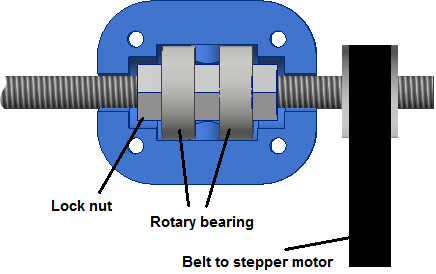
\includegraphics[width=7cm]{mech_bearings.png}
\end{center}
\caption{The `Bearing Block'.}
\label{fig:mech_bearings}
\end{figure}
With each of these components in place, the Wheel Unit comprises the wheel, motor, steering actuator and stepper motor, wishbones and suspension. This all-in-one unit, which can easily be removed from Tiberius' chassis, is identical in all four corners. This is a big step towards modularity of components, as every wheel unit is the same.
\newline
The completed design for the wheel mount unit, with suspension and steering actuator in place, is shown in Figure \ref{fig:mech_wheelmount}.
\newline
\begin{figure}[!htb]
\begin{center}
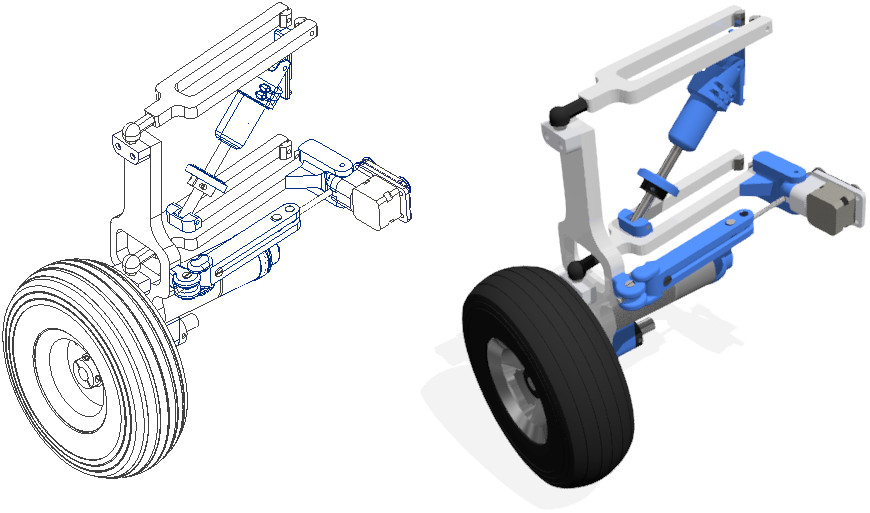
\includegraphics[width=14cm]{mech_wheel_mount.png}
\end{center}
\caption{The `Wheel Mount' assembly; design (left), colour render (right). 3D printed components in blue.}
\label{fig:mech_wheelmount}
\end{figure}

\subsection{Chassis}
\label{sec:mech_DI_Chassis}
With the drastic changes to Tiberius' wheel mounts, a re-design of the chassis was required. The double wishbone suspension system requires two vertical attachment points, so the new chassis would have to be fairly tall. Similarly the wishbones protrude almost 30cm out from the hinges; in order to keep the robot a reasonable width, they would have to be mounted as close to the centre of the chassis as possible.
\newline
While Tiberius II was low and wide, the new chassis for Tiberius III is designed to be tall and slim. This allows the wishbones to be mounted at the centre on two columns, leaving plentiful space in the middle for new components. Space has been left at the front and back above the bumpers; at the front for the new robotic arm, and at the back for the batteries.
\newline
The objective of reducing wasted material has truly been fulfilled; the new chassis uses 537cm of aluminium extrusion, some four metres less than Tiberius II, and therefore saving some weight. The chassis has a multitude of areas for components to be mounted: either side of the central area, on top and underneath, and even in the space inside the central square. Components can also be mounted on top of and beneath the bumpers, which have been left for the acoustic sensors.
\begin{figure}[!htb]
\begin{center}
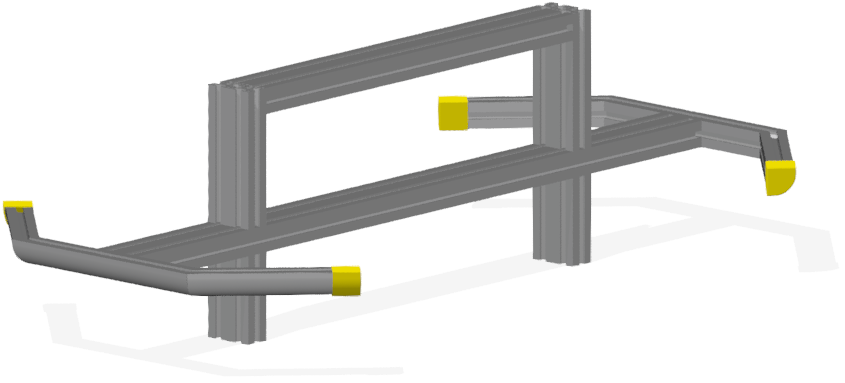
\includegraphics[width=10cm]{mech_frame.png}
\end{center}
\caption{Tiberius III's minimalistic aluminium frame, with all other components removed.}
\label{fig:mech_frame}
\end{figure}

\subsection{Motion}
% Covers all the stuff with Jim's mbeds

The new steering mechanics have introduced a new level of complexity to Tiberius's control software and hardware.

\subsubsection{Motor Control Architecture}
A new motor control subsystem has been introduced, introducing a \gls{canbus} network, a \gls{UDP} interface, whilst maintaining the existing \gls{i2c} interfaced MD03 motor drivers. \ref{fig:motor-control-architecture} illustrates the communications that exist in order to drive the wheel and steering motors.

The new control system will use a PID control loop, working with the rotary encoders to provide a controlled motor speed.

\begin{figure}[!htb]
\begin{center}
\includegraphics[width=11.5cm]{motor_control.png}
\end{center}
\caption{Motor Control Communication Architecture}
\label{fig:motor-control-architecture}
\end{figure}